% \newpage
\subsection{Hyperparameter Scaling}
\label{sec:hpscaling}

\paragraph{Motivation.}
\label{sec:hpscaling-motivation}
% Hyperparameters do not survive a change of architecture or optimizer
% The best learning rate and batch size depend on the model architecture and the optimizer, so a recipe that was optimal for the previous-generation model may become suboptimal once both change.
% % The observation that prompted the refit
% Under the hyperparameters of the Qwen3.5 scaling law~\citep{qwenteam2026qwen35}, the new architecture and optimizer trained noticeably more stably than before (\S\ref{sec:stability}), which suggested that the optimum had moved.

% % Background on what such a law predicts
% Both learning rate $\eta$ and batch size $B$ are usually described as power laws in the compute budget: the optimal learning rate falls and the optimal batch size grows as the budget increases~\citep{kaplan2020scaling}, with the batch size bounded above by a critical value beyond which extra data parallelism buys little~\citep{mccandlish2018largebatch,shallue2019dataparallelism,zhang2024criticalbatch}.

% % What the refit changed, and how the two predictions are checked
% We therefore refit the law. 
% Compared to the previous formulation, it predicts a substantially larger batch size and learning rate, as well as a slower decay of the learning rate as model size increases. 
% A law fitted at a small scale is only useful if its extrapolations hold. 
% Therefore, we validated the two predictions separately, testing each in the regime where its effects are most pronounced: we evaluated the batch size prediction on a small model trained for many tokens (where an excessively large batch size may lead to suboptimal performance), and the learning rate prediction on a large model trained with a limited compute budget (where training instability is the primary risk).

% (@Zihan Please review:)

% % Hyperparameters do not survive a change of architecture or optimizer

Choosing near-optimal hyperparameters is critical for efficient and stable model training. In previous generations of Qwen models, we fitted scaling laws for key hyperparameters, such as the learning rate ($\eta$) and batch size ($B$) \citep{qwen25, yang2025qwen3}. The optimal learning rate and batch size depend on the model architecture and the optimizer, so a recipe that was optimal for the previous-generation model may become suboptimal once both change.
% The observation that prompted the refit
Under our previous Qwen3.5 hyperparameter recipe~\citep{qwenteam2026qwen35}, we find that the new architecture and optimizer train noticeably more stably than before (\S\ref{sec:stability}), suggesting room for a more aggressive hyperparameter setting to further improve training performance.

Therefore, we develop an updated hyperparameter scaling law.
% Both learning rate ($\eta$) and batch size ($B$) are described as power laws of the number of model parameters and training tokens: the optimal learning rate falls and the optimal batch size grows as the budget increases~\citep{kaplan2020scaling}, with the batch size bounded above by a critical value beyond which extra data parallelism buys little~\citep{mccandlish2018largebatch,shallue2019dataparallelism,zhang2024criticalbatch}.
% What the refit changed, and how the two predictions are checked
% Compared to the previous formulation, it predicts a substantially larger batch size and learning rate, as well as a slower decay of the learning rate as model size increases, reflecting the changes in architecture and optimizer.
The architecture and optimizer changes shift the predicted near-optimal hyperparameters toward substantially larger batch sizes and learning rates, with a slower decay in the learning rate as model size increases.


A scaling law fitted at small scales is only useful if it extrapolates reliably.
We validated the learning-rate and batch-size predictions separately, evaluating each in a regime designed to make its effect more pronounced: the batch size prediction on a small model trained for many tokens (where an excessively large batch size may lead to suboptimal performance), and the learning rate prediction on a large model trained for a limited token budget (where training instability is the primary risk).
The predicted hyperparameters lie in the near-optimal basin and yield clear improvements over the previous Qwen3.5 recipe in both pretraining loss and benchmark performance.

\begin{figure}[t]
  \centering
  \vskip -0.2in
  \begin{subfigure}[t]{0.49\linewidth}
    \centering
    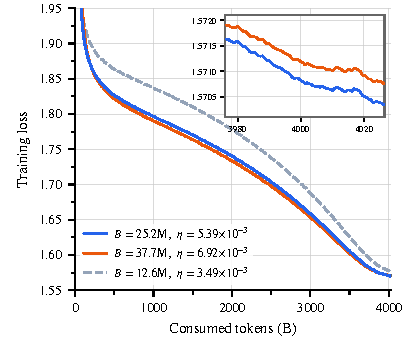
\includegraphics[pagebox=cropbox,width=\linewidth]{figs/paper_bsz_compare_half.pdf}
    \vskip -0.05in
    \caption{Constant batch size.}
    \label{fig:hp-bsz-compare}
  \end{subfigure}
  \hfill
  \begin{subfigure}[t]{0.49\linewidth}
    \centering
    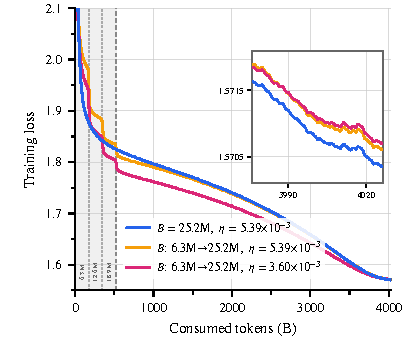
\includegraphics[pagebox=cropbox,width=\linewidth]{figs/paper_bsz_warmup_loss_half.pdf}
    \vskip -0.05in
    \caption{Ramped batch size.}
    \label{fig:hp-bsz-warmup}
  \end{subfigure}
  \vskip -0.05in
  \caption{\textbf{Batch size on a 4T-token budget.} Training loss against consumed tokens for a 20-layer 10.8B-A0.89B MoE; each inset resolves the last 50B tokens. 
  \textbf{(a)} Moving from the previous recipe ($B\,{=}\,12.6$M) to the predicted optimum ($B\,{=}\,25.2$M) is worth $7.2\times10^{-3}$, while a further step to $B\,{=}\,37.7$M leads to a minor degradation. The loss rises steeply below the prediction and remains nearly flat above it.
  \textbf{(b)} Reaching $B\,{=}\,25.2$M through a ramp instead performs no better than using this batch size from the start and takes $18.8\%$ more optimizer steps.}
\end{figure}

\paragraph{Batch Size at a Large Token Budget.}
\label{sec:hpscaling-bsz}
% Setup
The batch-size prediction is evaluated on a 20-layer 10.8B-A0.89B MoE model trained over $4$T tokens.
We compare the previous recipe ($B\,{=}\,12.6$M), the optimum predicted by the new scaling law ($B\,{=}\,25.2$M), and a setting $1.5\times$ larger ($B\,{=}\,37.7$M), with each configuration using the learning rate prescribed by the scaling law for its respective batch size.
All runs consume the same token budget, ensuring the comparison is based on equal compute.

% Result
Averaged over the final 20B tokens, the losses are $1.5702$ at $B\,{=}\,25.2$M , $1.5707$ at $B\,{=}\,37.7$M, and $1.5774$ under the previous recipe (Fig.~\ref{fig:hp-bsz-compare}).
The new scaling-law fit therefore improves the loss by $7.2\times10^{-3}$ over the previous recipe, while a further $1.5\times$ increase in batch size incurs a $4.3\times10^{-4}$ penalty, which is not significant.
The loss increases sharply below the predicted batch size and plateaus above it, indicating that the prediction is close to optimal and large enough to realize performance gains without being excessive.



\paragraph{Batch-Size Warmup Is No Longer Necessary.}
\label{sec:hpscaling-warmup}

% The practice and the usual arguments for it
Large runs commonly ramp the batch size over early training rather than starting at its final value~\citep{brown2020gpt3,liu2024deepseek}. 
The rationale is that the critical batch size is small early in training and grows over time~\citep{mccandlish2018largebatch,zhang2024criticalbatch}, making a large batch inefficient at the start. 
Furthermore, smaller batches paired with a scaled learning rate~\citep{goyal2017minibatch} are generally easier to stabilize during the initial steps.

% Why we re-tested it: our observations with Muon and MoE
However, our previous hyperparameter sweep suggests a different behavior when using the Muon optimizer. 
We observe that decreasing the batch size below the predicted optimum incurs a more significant performance penalty than increasing it, and that Muon preserves data efficiency at larger batch sizes where AdamW's performance degrades~\citep{jordan2024muon,essentialai2025muon}. 
For sparse MoE models, a larger batch also ensures that every expert receives a sufficient and diverse token signal per step, which plausibly aids expert specialization~\citep{global_balance}. 
Together, these observations led us to hypothesize that batch-size warmup may be unnecessary.


% Setup
We therefore re-tested the batch-size warmup. 
We increase the batch size from $6.3$M in increments of $6.3$M, reaching the target of $25.2$M at 524B tokens. 
We evaluated two variants: the first maintains the peak learning rate of the constant-batch optimum, making the ramp its only difference; the second lowers the peak learning rate to account for the smaller batch sizes in the early stages.

% Result
Neither variant improves performance (Fig.~\ref{fig:hp-bsz-warmup}). 
Both ramps converge within the run-to-run variance but remain slightly worse than the constant-batch baseline, underperforming by $2.5\times10^{-4}$ and $3.5\times10^{-4}$, respectively. 
Additionally, the warmup requires $18.8\%$ more optimizer steps for the same token budget, resulting in greater wall-clock time overhead. 
Training stability is also unaffected: no run in this sweep exhibits a step where the loss exceeds its local median by more than $0.1$, and the p99.9 pre-clip gradient norm ranges from $0.088$ to $0.190$, well below the clipping threshold of $0.5$.

% Mechanism and Trajectory
The loss trajectory of the warmup runs reveals the underlying mechanism. 
During the warmup phase, the smaller batch size introduces higher gradient noise under the same learning rate, resulting in a higher loss compared to the constant-batch baseline. 
Shortly after the batch size reaches its target, the warmup variant may exhibit a transient loss advantage due to the greater number of optimization steps accumulated during the early phase. 
However, as the learning rate decays and the model approaches convergence, this step-count advantage is neutralized. 
Ultimately, the constant-batch baseline surpasses the warmup runs, yielding a better final loss. 
Consequently, we do not employ batch-size warmup in our production runs.


\begin{figure}[h]
  \centering
  \begin{subfigure}[t]{0.49\linewidth}
    \centering
    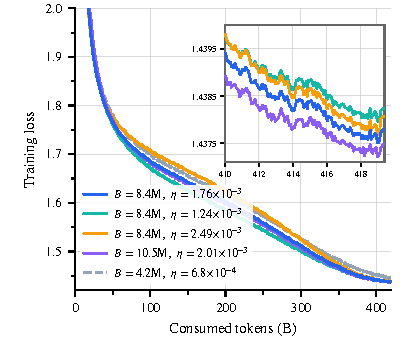
\includegraphics[pagebox=cropbox,width=\linewidth]{figs/paper_lr_lm_loss_half.pdf}
    \vskip -0.05in
    \caption{Training loss.}
    \label{fig:hp-lr-loss}
  \end{subfigure}
  \hfill
  \begin{subfigure}[t]{0.49\linewidth}
    \centering
    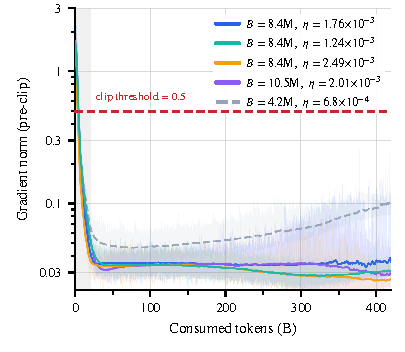
\includegraphics[pagebox=cropbox,width=\linewidth]{figs/paper_lr_grad_norm_half.pdf}
    \vskip -0.05in
    \caption{Gradient norm.}
    \label{fig:hp-lr-gnorm}
  \end{subfigure}
  \vskip -0.05in
  \caption{\textbf{Learning rate at a larger model scale.} Five runs of a
    48-layer MoE on a 419B-token budget: the predicted optimum ($B\,{=}\,8.4$M,
    $\eta\,{=}\,1.76\times10^{-3}$), $\eta$ divided and multiplied by $\sqrt{2}$,
    a $25\%$ larger batch with its matched $\eta$, and the previous recipe
    (dashed). \textbf{(a)} The inset covers the last 10B tokens. The loss differences among the predicted optimum and the three nearby settings are near the noise level, so the predicted optimum sits at the bottom of a flat bowl. 
    \textbf{(b)} Pre-clip gradient norm on a log scale, with individual steps faint behind a moving average, the warmup shaded
    and the clip threshold dashed. After warmup, the pre-clip gradient norms of all runs near the predicted optimum remain below $50\%$ of the clipping threshold, including the run at $\sqrt{2}$ times the predicted learning rate.}
\end{figure}


\paragraph{Learning Rate at a Larger Model Scale.}
\label{sec:hpscaling-lr}
% Setup
The learning-rate prediction is tested on a much larger $48$ layers 156B-A7B MoE, over a $419$B-token budget that is again the same for every run.
We evaluate the predicted optimum together with learning rates scaled by $1/\sqrt{2}$ and $\sqrt{2}$, a $25\%$ larger batch with its matched learning rate, and the previous hyperparameter recipe.

% Result 1: the endpoint is invariant, and the old recipe is not

The previous recipe ends $7.8\times10^{-3}$ above the predicted optimum, while the four settings near the predicted optimum end within $7\times10^{-4}$ of each other, near the noise level (Fig.~\ref{fig:hp-lr-loss}).
The optimum therefore sits at the bottom of a bowl that is flat over at least a factor of $\sqrt{2}$ in either direction in learning rate and $+25\%$ in batch size; the larger batch is nominally the best of the four, by $3\times10^{-4}$.


\begin{table*}[t]
\vskip -0.2in
\centering
\small
\setlength{\tabcolsep}{3.5pt}
\caption{Downstream accuracy of the five learning-rate runs of
Fig.~\ref{fig:hp-lr-loss}, all at the same $419$B-token budget on the 48-layer 156B-A7B MoE. 
All values are percentages and higher is better; the benchmarks and the evaluation pipeline are those of \S\ref{sec:gdn-ablation}. 
Bold denotes the best result in each column.}
\vskip -0.05in
\label{tab:hp-lr-bench}
\resizebox{\textwidth}{!}{%
\begin{tabular}{lcccccccccc}
\toprule
& & & \multicolumn{3}{c}{Knowledge} & \multicolumn{2}{c}{STEM} & Reasoning & Multilingual & \\
\cmidrule(lr){4-6} \cmidrule(lr){7-8} \cmidrule(lr){9-9} \cmidrule(lr){10-10}
% Setting & $B$ & $\eta$ & MMLU & MMLU-Pro & SuperGPQA & MATH & GSM8K & BBH & MMMLU & Avg. \\
Setting
& \multicolumn{1}{c}{$B$}
& \multicolumn{1}{c}{$\eta$}
& \multicolumn{1}{c}{MMLU}
& \multicolumn{1}{c}{MMLU-Pro}
& \multicolumn{1}{c}{SuperGPQA}
& \multicolumn{1}{c}{MATH}
& \multicolumn{1}{c}{GSM8K}
& \multicolumn{1}{c}{BBH}
& \multicolumn{1}{c}{MMMLU}
& \multicolumn{1}{c}{Avg.} \\
\midrule
New fit, predicted optimum
& $8.4$M & $1.76\times10^{-3}$
& \textbf{73.84} & 48.35 & \textbf{29.31} & \textbf{49.98} & \textbf{80.89} & 73.25 & 68.23 & \textbf{60.55} \\
New fit, $\eta\div\sqrt{2}$
& $8.4$M & $1.24\times10^{-3}$
& 73.59 & 47.00 & 28.10 & 48.92 & 77.48 & 72.00 & 66.88 & 59.14 \\
New fit, $\eta\times\sqrt{2}$
& $8.4$M & $2.49\times10^{-3}$
& \textbf{73.84} & 46.92 & 28.04 & 49.58 & 80.06 & \textbf{73.82} & \textbf{68.46} & 60.10 \\
New fit, $B\times1.25$
& $10.5$M & $2.01\times10^{-3}$
& 73.73 & \textbf{48.51} & 28.52 & 49.32 & 80.06 & 72.58 & 67.72 & 60.06 \\
Qwen3.5 recipe
& $4.2$M & $6.8\times10^{-4}$
& 71.23 & 45.35 & 25.67 & 45.54 & 74.32 & 69.54 & 63.19 & 56.41 \\
\bottomrule
\end{tabular}
}
\end{table*}

Downstream benchmark results demonstrate the robust convergence achieved by our new scaling-law fit (Tab.~\ref{tab:hp-lr-bench}). 
The predicted optimum yields the highest average accuracy, securing the best or tied-best scores across the majority of evaluated tasks, while the previous recipe falls noticeably behind. 
Crucially, increasing the batch size or learning rate beyond the predicted optimum results in only a marginal, statistically insignificant drop in benchmark performance. 
This indicates a highly stable optimization landscape where the model's generalization does not sharply degrade with slight hyperparameter deviations. 
We treat these specific rankings as observational; given the single evaluation per run and the narrow margins among the top settings, these minor variations likely fall within standard evaluation noise.

Beyond final performance, maintaining training stability is paramount at large model scales.
The training dynamics remain exceptionally stable across all configurations. 
Gradient clipping never engages after the warmup phase in any of the five runs. 
At the predicted optimum, the maximum pre-clip gradient norm reaches only $28\%$ of the clipping threshold, compared to $51\%$ under the previous recipe, which suffers from noisier gradients due to its smaller batch size (Fig.~\ref{fig:hp-lr-gnorm}). 
Furthermore, the loss curves are remarkably smooth without any loss spike; no run exhibits a single step where the loss exceeds its local median by more than $0.1$. 
Even further increasing the predicted learning rate at this scale remains entirely stable. 
This confirms that our new scaling law does not dangerously over-extrapolate, providing an efficient, safe and robust hyperparameter recipe for large-scale training.

